\section{Architecture}

The architecture used on this project is the integration of three systems: Robot Shop \cite{robotshop}, ELK \cite{elk}, and MLog \cite{mlog}.

\begin{figure}[htbp]
\centering
\centerline{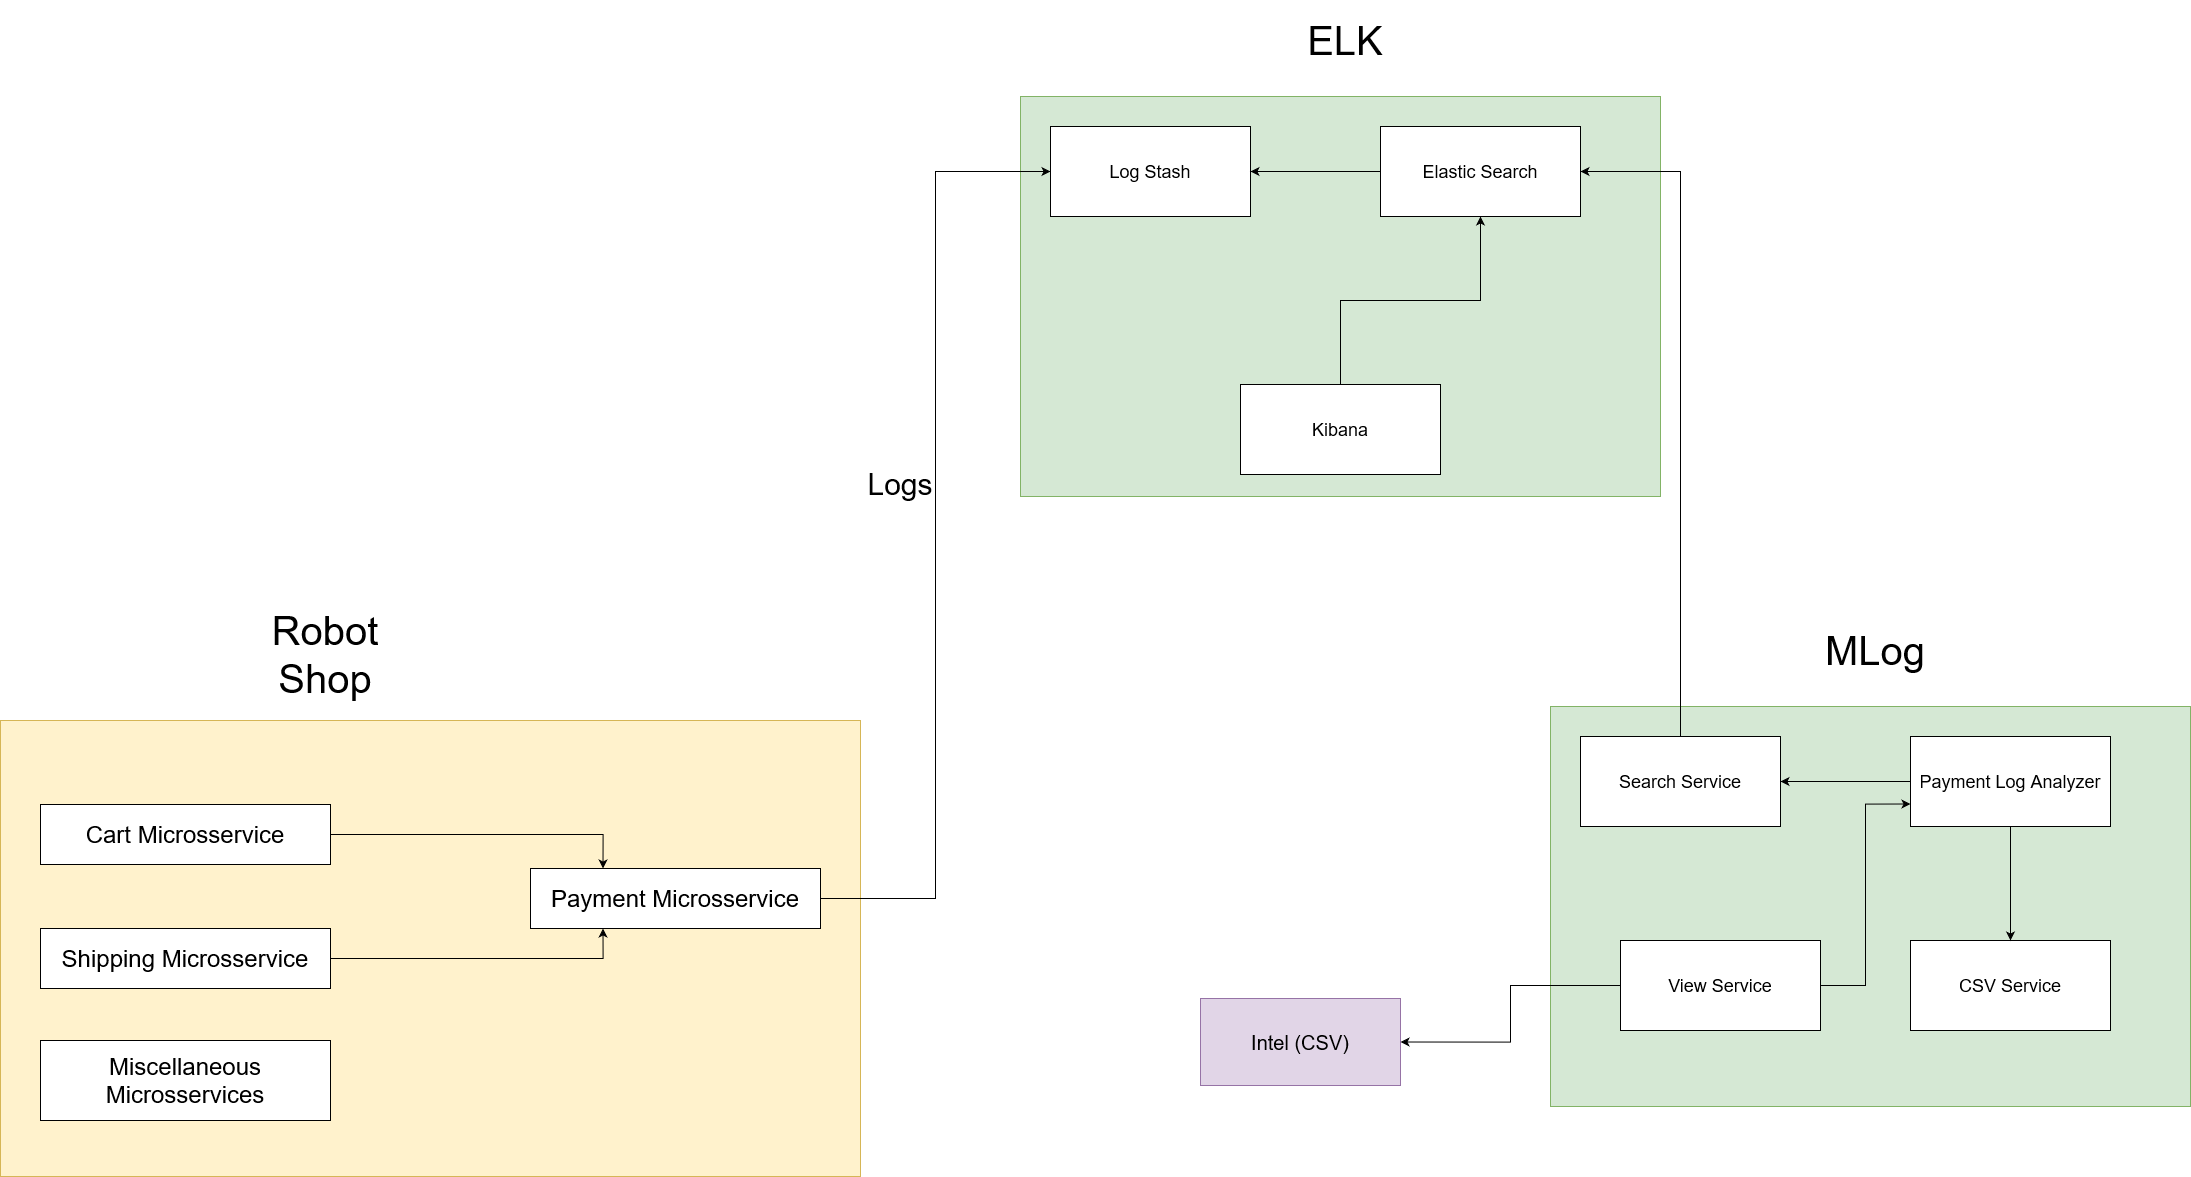
\includegraphics[width=0.5\textwidth]{Media/architecture.png}}
\caption{A generalized view of this project is architecture.}
\label{fig:architecture}
\end{figure}

\subsection{Robot Shop}

The e-commerce that has the logs analyzed on this paper is the Robot Shop \cite{robotshop}, it is a simple microservices-based e-commerce with open source. There are 12 services on the Robot Shop, but the information analyzed is contained on the payment microservice, as this service carries the data of both shipping and cart services, on purchase.

\begin{figure}[htbp]
\centering
\centerline{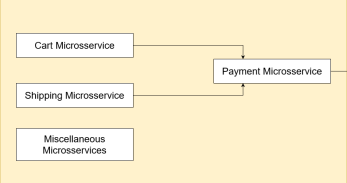
\includegraphics[width=0.5\textwidth]{Media/robot_shop.png}}
\caption{The Robot Shop is architecture}
\label{fig:architecture-robot-shop}
\end{figure}

\subsection{ELK}

ELK \cite{elk} is a project that groups kibana \cite{kibana}, elastic search \cite{elasticsearch} and logstash \cite{logstash}. The logs generated on the payment microservice are sent and stored on logstash. After creating an index pattern on kibana, it is possible to see the logs store on logstash through kibana is interface. ELK also has the elastic search service, which can search through the stored logs to analyze the data contained on the payment is logs.

\begin{figure}[htbp]
\centering
\centerline{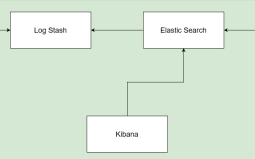
\includegraphics[width=0.5\textwidth]{Media/elk.png}}
\caption{The ELK is architecture}
\label{fig:architecture-elk}
\end{figure}

\subsection{MLog}

MLog \cite{mlog} is the project developed with this paper, and it consists on 4 services:

\begin{itemize}
  \item The view service, which is the front-end of MLog, it enables the filter and download of the analysis.
  \item The payment log analyzer service is the service that receives the data on the logs to find valuable information. This service is also responsible for receiving the request from the view service, for requesting the data from the search service, and for requesting the download of the CSV contained the data analyzed.
  \item Search service is the service that requests the queries to elastic search, it also filters the logs further to get only the data about the purchase.
  \item CSV service is a common service that generates a CSV file based on the data passed on the request.
\end{itemize}

\begin{figure}[htbp]
\centering
\centerline{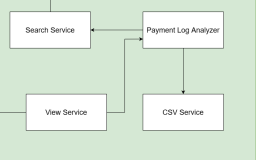
\includegraphics[width=0.5\textwidth]{Media/mlog.png}}
\caption{The MLog is architecture}
\label{fig:architecture-mlog}
\end{figure}